% Options for packages loaded elsewhere
\PassOptionsToPackage{unicode}{hyperref}
\PassOptionsToPackage{hyphens}{url}
%
\documentclass[
  11pt,
  landscape]{article}
\usepackage{lmodern}
\usepackage{amssymb,amsmath}
\usepackage{ifxetex,ifluatex}
\ifnum 0\ifxetex 1\fi\ifluatex 1\fi=0 % if pdftex
  \usepackage[T1]{fontenc}
  \usepackage[utf8]{inputenc}
  \usepackage{textcomp} % provide euro and other symbols
\else % if luatex or xetex
  \usepackage{unicode-math}
  \defaultfontfeatures{Scale=MatchLowercase}
  \defaultfontfeatures[\rmfamily]{Ligatures=TeX,Scale=1}
  \setsansfont[]{Calibri Light}
\fi
% Use upquote if available, for straight quotes in verbatim environments
\IfFileExists{upquote.sty}{\usepackage{upquote}}{}
\IfFileExists{microtype.sty}{% use microtype if available
  \usepackage[]{microtype}
  \UseMicrotypeSet[protrusion]{basicmath} % disable protrusion for tt fonts
}{}
\makeatletter
\@ifundefined{KOMAClassName}{% if non-KOMA class
  \IfFileExists{parskip.sty}{%
    \usepackage{parskip}
  }{% else
    \setlength{\parindent}{0pt}
    \setlength{\parskip}{6pt plus 2pt minus 1pt}}
}{% if KOMA class
  \KOMAoptions{parskip=half}}
\makeatother
\usepackage{xcolor}
\IfFileExists{xurl.sty}{\usepackage{xurl}}{} % add URL line breaks if available
\IfFileExists{bookmark.sty}{\usepackage{bookmark}}{\usepackage{hyperref}}
\hypersetup{
  hidelinks,
  pdfcreator={LaTeX via pandoc}}
\urlstyle{same} % disable monospaced font for URLs
\usepackage[margin=1in]{geometry}
\usepackage{graphicx,grffile}
\makeatletter
\def\maxwidth{\ifdim\Gin@nat@width>\linewidth\linewidth\else\Gin@nat@width\fi}
\def\maxheight{\ifdim\Gin@nat@height>\textheight\textheight\else\Gin@nat@height\fi}
\makeatother
% Scale images if necessary, so that they will not overflow the page
% margins by default, and it is still possible to overwrite the defaults
% using explicit options in \includegraphics[width, height, ...]{}
\setkeys{Gin}{width=\maxwidth,height=\maxheight,keepaspectratio}
% Set default figure placement to htbp
\makeatletter
\def\fps@figure{htbp}
\makeatother
\setlength{\emergencystretch}{3em} % prevent overfull lines
\providecommand{\tightlist}{%
  \setlength{\itemsep}{0pt}\setlength{\parskip}{0pt}}
\setcounter{secnumdepth}{-\maxdimen} % remove section numbering
\usepackage{floatrow}
\usepackage{caption}
\usepackage{subcaption}
\usepackage{background}
\usepackage{titling}
\usepackage{xcolor}
\usepackage{graphicx}
\usepackage{tikz}
\usepackage[most]{tcolorbox}
\usetikzlibrary{calc}
\usepackage{caption}
\usepackage{background}
\usepackage{subcaption}
\usepackage[absolute,overlay]{textpos}
\pretitle{\begin{flushleft}}
\posttitle{\end{flushleft}}
\definecolor{amethyst}{RGB}{123, 186, 233}
\color{black}
\geometry{top=0.75in,left=0.80in,bottom=0.75in,right=0.80in}

\author{}
\date{\vspace{-2.5em}}

\begin{document}

\thispagestyle{empty}

\begin{tikzpicture}[overlay, remember picture]
\node[anchor=west, %anchor is upper left corner of the graphic
      xshift=0cm, %shifting around
      yshift=0cm] 
     at (current page.west) %left upper corner of the page
     {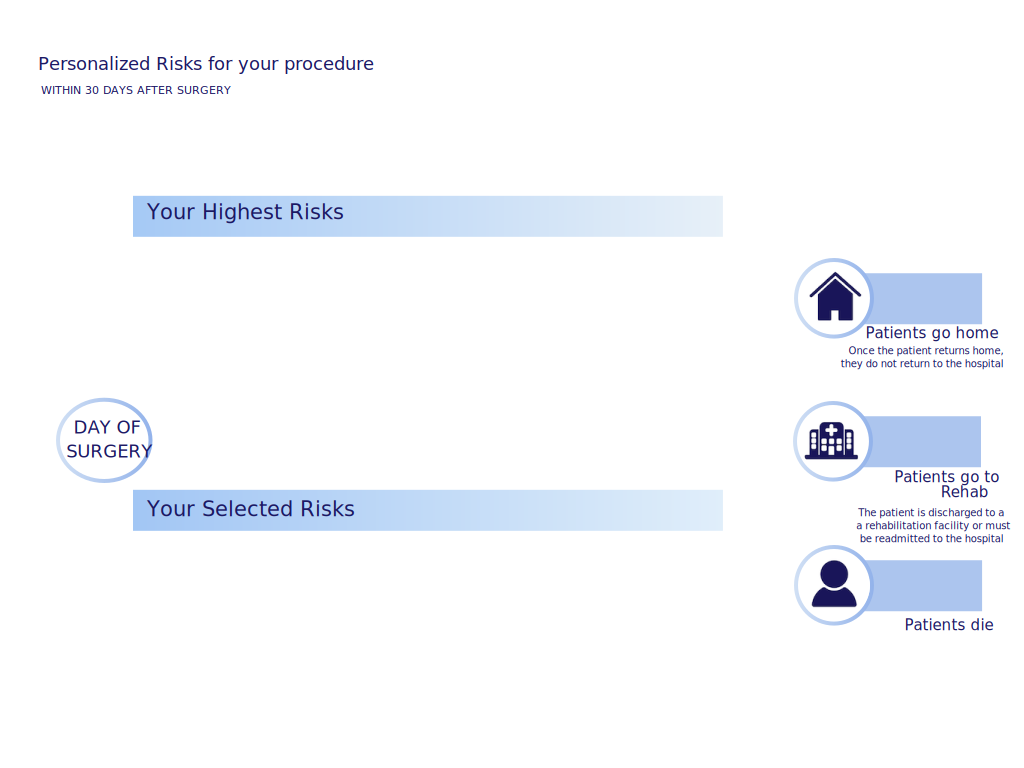
\includegraphics[width=\paperwidth,height=\paperheight]{"New Images/Background_1.png"}}; 
\end{tikzpicture}

\begin{tikzpicture}[overlay, remember picture]
\node[anchor=west, %anchor is upper left corner of the graphic
      xshift=0cm, %shifting around
      yshift=0cm] 
     at (current page.west) %left upper corner of the page
     {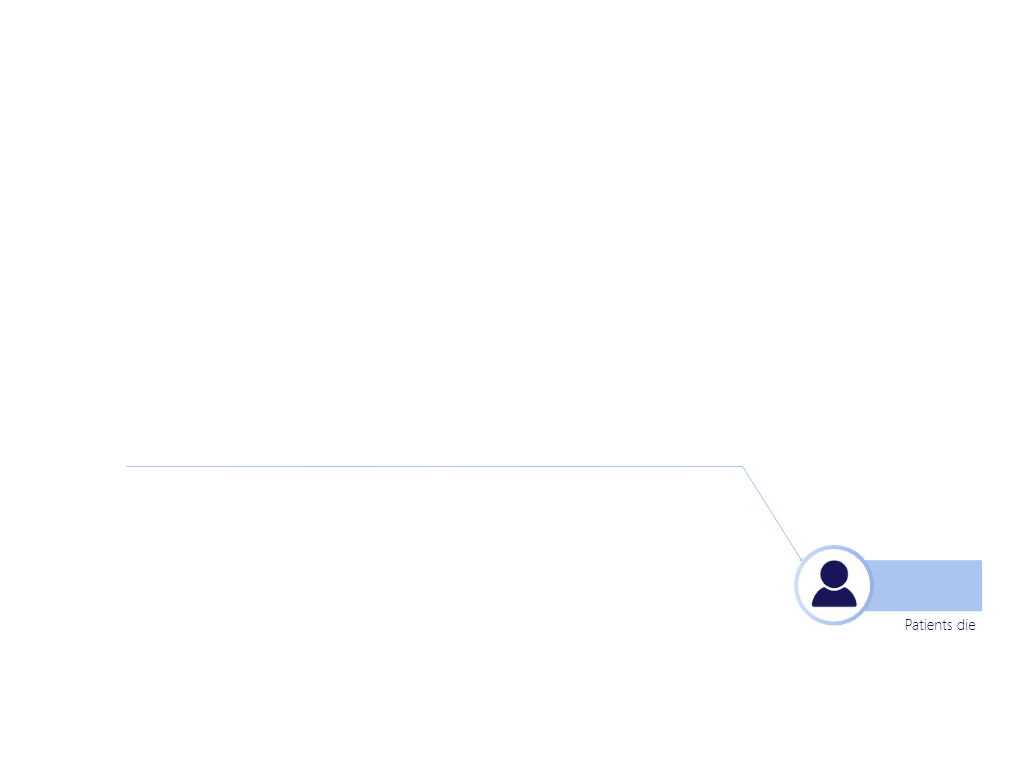
\includegraphics[width=\paperwidth,height=\paperheight]{New Images/bot1.png}}; 
\end{tikzpicture}

\begin{tikzpicture}[overlay, remember picture]
\node[anchor=west, %anchor is upper left corner of the graphic
      xshift=0cm, %shifting around
      yshift=0cm] 
     at (current page.west) %left upper corner of the page
     {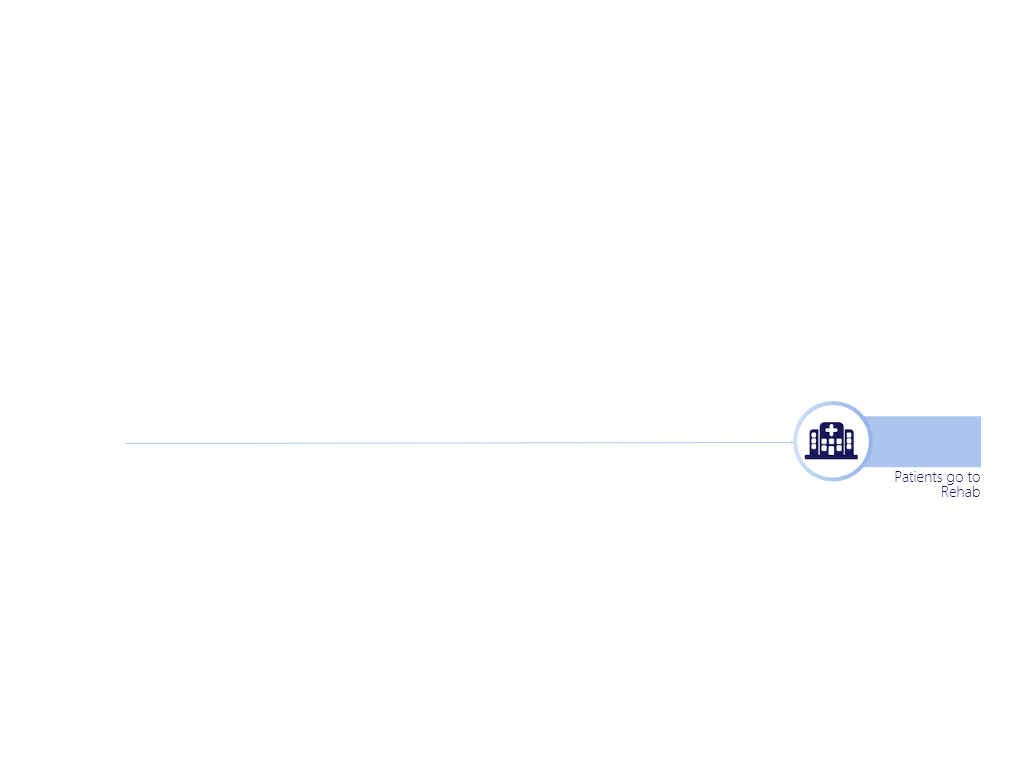
\includegraphics[width=\paperwidth,height=\paperheight]{New Images/middle1.png}}; 
\end{tikzpicture}

\begin{tikzpicture}[overlay, remember picture]
\node[anchor=west, %anchor is upper left corner of the graphic
      xshift=0cm, %shifting around
      yshift=0cm] 
     at (current page.west) %left upper corner of the page
     {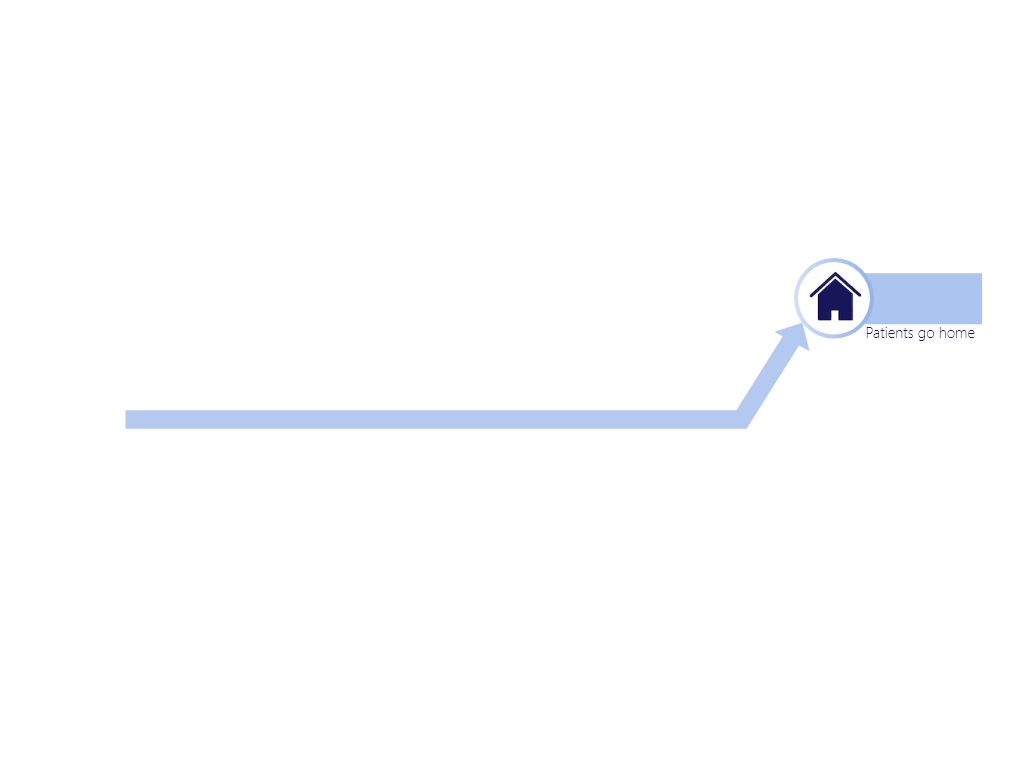
\includegraphics[width=\paperwidth,height=\paperheight]{New Images/top5.png}}; 
\end{tikzpicture}

\begin{tikzpicture}[overlay, remember picture]
\node[anchor=west, %anchor is upper left corner of the graphic
      xshift=0cm, %shifting around
      yshift=0cm] 
     at (current page.west) %left upper corner of the page
     {\includegraphics[width=\paperwidth,height=\paperheight]{"New Images/background_3.png"}}; 
\end{tikzpicture}

\begin{textblock*}{5cm}(3.9cm,9.4cm) % {block width} (coords) 
    \centerline{\small{Infection}}
\end{textblock*}

\begin{textblock*}{5cm}(3.9cm,9.9cm) % {block width} (coords) 
    \small \centerline{\textit{Average}}
\end{textblock*}

\begin{textblock*}{5cm}(3.9cm,10.3cm) % {block width} (coords) 
    \centerline{\textbf{3.21\%}}
\end{textblock*}

\begin{textblock*}{5cm}(9.4cm,9.4cm) % {block width} (coords) 
    \centerline{\small{Urinary Tract Infection}}
\end{textblock*}

\begin{textblock*}{5cm}(9.4cm,9.9cm) % {block width} (coords) 
    \small \centerline{\textit{Average}}
\end{textblock*}

\begin{textblock*}{5cm}(9.4cm,10.3cm) % {block width} (coords) 
    \centerline{\textbf{1.23\%}}
\end{textblock*}

\begin{textblock*}{5cm}(14.9cm,9.4cm) % {block width} (coords) 
    \centerline{\small{Venous thromboembolism}}
\end{textblock*}

\begin{textblock*}{5cm}(14.9cm,9.9cm) % {block width} (coords) 
    \small \centerline{\textit{Average}}
\end{textblock*}

\begin{textblock*}{5cm}(14.9cm,10.3cm) % {block width} (coords) 
    \centerline{\textbf{0.65\%}}
\end{textblock*}

\begin{textblock*}{5cm}(3.9cm,17.55cm) % {block width} (coords) 
    \centerline{\small{Respiratory Complications}}
\end{textblock*}

\begin{textblock*}{5cm}(3.9cm,18.05cm) % {block width} (coords) 
    \small \centerline{\textit{Average}}
\end{textblock*}

\begin{textblock*}{5cm}(3.9cm,18.4cm) % {block width} (coords) 
    \centerline{\textbf{0.61\%}}
\end{textblock*}

\begin{textblock*}{5cm}(9.4cm,17.55cm) % {block width} (coords) 
    \centerline{\small{Renal Complications}}
\end{textblock*}

\begin{textblock*}{5cm}(9.4cm,18.05cm) % {block width} (coords) 
    \small \centerline{\textit{Average}}
\end{textblock*}

\begin{textblock*}{5cm}(9.4cm,18.4cm) % {block width} (coords) 
    \centerline{\textbf{0.23\%}}
\end{textblock*}

\begin{textblock*}{5cm}(14.9cm,17.55cm) % {block width} (coords) 
    \centerline{\small{Cardiac Complications}}
\end{textblock*}

\begin{textblock*}{5cm}(14.9cm,18.05cm) % {block width} (coords) 
    \small \centerline{\textit{Average}}
\end{textblock*}

\begin{textblock*}{5cm}(14.9cm,18.4cm) % {block width} (coords) 
    \centerline{\textbf{0.11\%}}
\end{textblock*}

\begin{textblock*}{2.4cm}(24.5cm,8.2cm) % {block width} (coords) 
  \huge \textcolor{black}{\textbf{0.98} \huge \%}
\end{textblock*}

\begin{textblock*}{2.4cm}(24.5cm,12.1cm) % {block width} (coords) 
  \huge \textcolor{black}{\textbf{0.01} \huge \%}
\end{textblock*}

\begin{textblock*}{2.4cm}(24.5cm,16cm) % {block width} (coords) 
  \huge \textcolor{black}{\textbf{0.00} \huge \%}
\end{textblock*}

\vspace{2.75em}

\begin{figure}
 \hspace{-4.24cm}
 \begin{subfloatrow}%

\ffigbox[20cm][]{%
 \begin{subfloatrow}[3]%
 \ffigbox[5.3cm][]{%

\begin{center}
\includegraphics{download_handler_files/figure-latex/unnamed-chunk-1-1} \end{center}
    }{{}}

    \ffigbox[5cm][]{%

\begin{center}
\includegraphics{download_handler_files/figure-latex/unnamed-chunk-2-1} \end{center}
    }{{}}
    
    \ffigbox[5.2cm][]{%

\begin{center}
\includegraphics{download_handler_files/figure-latex/unnamed-chunk-3-1} \end{center}
    }{{}}
      
    \end{subfloatrow}
  }{
   
  }
  \end{subfloatrow}
\end{figure}

\vspace{4.48cm}

\begin{figure}
 \hspace{-4.24cm}
 \begin{subfloatrow}%

\ffigbox[20cm][]{%
 \begin{subfloatrow}[3]%
 \ffigbox[5.3cm][]{%

\begin{center}
\includegraphics{download_handler_files/figure-latex/unnamed-chunk-4-1} \end{center}
    }{{}}

    \ffigbox[5cm][]{%

\begin{center}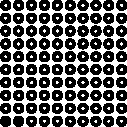
\includegraphics{download_handler_files/figure-latex/unnamed-chunk-5-1} \end{center}
    }{{}}
    
    \ffigbox[5.2cm][]{%

\begin{center}
\includegraphics{download_handler_files/figure-latex/unnamed-chunk-6-1} \end{center}
    }{{}}
      
    \end{subfloatrow}
  }{
   
  }
  \end{subfloatrow}
\end{figure}

\begin{flushright}
\vspace{-16.5cm} \hspace{18cm} \normalsize Date Calculated:

\vspace{-0.25 cm} \hspace{18cm} \normalsize \textbf{12/12/12}

\vspace{-0.2cm} \hspace{18cm} \normalsize For the following procedure

\vspace{-0.2cm} \hspace{18cm} \small \textbf{52240}

\vspace{-0.2cm} \hspace{18cm} \normalsize With the following profile:

\vspace{-0.2cm} \hspace{18cm} \small \textbf{Male, Acites, Current Smoker}
\end{flushright}

\end{document}
